\section{Preliminares}
Vamos a dejar las formulas que mas se utilizan en los finales 

\subsection{PVI - orden = 1}
\subsubsection{Euler implicito}
$$
    y_{n+1} = y_n + h  f(y_n, t_n)
$$
¿Qué es cada cosa?

 \begin{enumerate}
     \item {$y_n$} es el valor aproximado de $y$
     \item {$y_{n+1}$} es el valor aproximado de $y$ en el siguiente paso 
     \item {$h$} es el tamaño del paso (incremento de $t$) 
     \item {$f(y_n, t_n)$} es la función que define la EDO $y' = f(y,t)$
 \end{enumerate}


\subsubsection{Ejemplos}
Dada la siguiente ecuación diferencial: 
$$y' = -y + t +1$$
Sabiendo que $y(0) = 1$

\begin{enumerate}
    \item {Calcular $u(t=1)$ con un solo avance}
    \item {Calcular $u(t=1)$ con 2 avances}
\end{enumerate} 


Para el punto 1, lo que hacemos es identificar cada termino de nuestra EDO sobre la expresión de euler implicito. 

\begin{itemize}

    \item {$f(y_n, t_n) = -y + t + 1$}
\end{itemize}

Reescribimos la formula de euler con nuestros datos. 

$$ 
y_{n+1} = y_n + h  (-y + t + 1)
$$


Para el punto 2, solamente hay que hacer 1 iteración con $t = 1$ y con $h = 1$

Calculamos $y_1$. 

$$
f(y_0, t_0) = -y_0+ t_0 + 1 = -1 + 0 + 1 = 0 
$$

Por lo tanto nos quedaría que

$$y_1 = 1 + 1*0 $$
$$y_1 = 1  $$

Entonces, con un solo avance de $h = 1$, calculamos $u(t = 1)$ y obtenemos que $u(1) = y_1 = 1$

Para el punto 2 hay que hacer lo mismo pero 2 iteraciones.
\subsubsection{Euler explicito}
$$
    y_{n+1} = y_n + h  f(y_{n + 1}, t_{n + 1})
$$
\subsubsection{Runge-Kutta de orden 2 }
$$
    q_{1u} = h  f(u_{n}, t_{n})
$$
$$
    q_{2u} = h  f(u_{n} + q_{1u}, t_{n + 1})
$$
$$
    u_{n+1} = u_n + \frac{1}{2}  (q_{1u} + q_{2u})
$$
\subsubsection{Runge-Kutta de orden 4}
\begin{align*}
q_{1_u} &= h \cdot f(u_n, t_n) \\
q_{2_u} &= h \cdot f\left(u_n + \frac{1}{2} q_{1_u}, t_n + \frac{1}{2} h\right) \\
q_{3_u} &= h \cdot f\left(u_n + \frac{1}{2} q_{2_u}, t_n + \frac{1}{2} h\right) \\
q_{4_u} &= h \cdot f\left(u_n + q3_u, t_n + h\right) \\
u_{n+1} &= u_n + \frac{1}{6} \left(q_{1_u} + 2q_{2_u} + 2q_{3_u} + q_{4_u}\right)
\end{align*}


\subsubsubsection{Observación}

Generalmente en el final te dan las formulas que vas a usar. En la gran mayoria de los casos, RK4 no lo usas ya que es eterno, a lo mejor te piden una iteración, pero no vi muchos finales que te lo pidan.

\subsection{PVI - orden mayor o igual 2 }

\begin{equation}
\left\{
\begin{array}{l}
u' = f(t,u,v) \\
v' = g(t,u,v)
\end{array}
\right.
\end{equation}

Esto queda más claro con ejercicios, tranqui que lo vamos a ver y a usar. 

\subsection{PVC}
\subsubsection{Diferencias finitas para problemas lineales}

Teniendo un problema del estilo: 


$$y'' = p(x)y' + q(x) + r(x) $$

para $a \leq x \leq b$ con $y(a) = \alpha$, $y(b) = \beta$


Al usar diferencias centradas de orden 2:

$$
y''(x_i) = \frac{y(x_{i+1}) - 2y(x_i) + y(x_{i-1}) }{h^2}
$$
$$
y'(x_i) = \frac{y(x_{i + 1}) - y(x_{i-1})}{2h}
$$

Se construye un sistema de ecuaciones lineales.

Primero vamos a hacer un cambio de variables: 

$$w_0 = \alpha, \space w_{N + 1} = \beta$$

Lo que hacemos es despejar $r(x)$, lo cual nos queda:

$$-r(x) = \frac{-w{i+1} + 2w(x_i) - w_{i-1} }{h^2} + p(x)(\frac{w_{i + 1} - w_{i - 1}}{2h}) + q(x_i)w_i $$



$$-h^2r(x) = -(1 + \frac{h}{2} p(x_i))w_{i -1} + (2 + h^2 q(x_i))w_i - (1 - \frac{h}{2} p(x_i))w_{i + 1}$$


Resulta un sistema tridiagonal $N \times N$, $Aw = b$


Ese sistema es medio un quilombo y queda asi

\begin{figure}[ht]
    \centering
    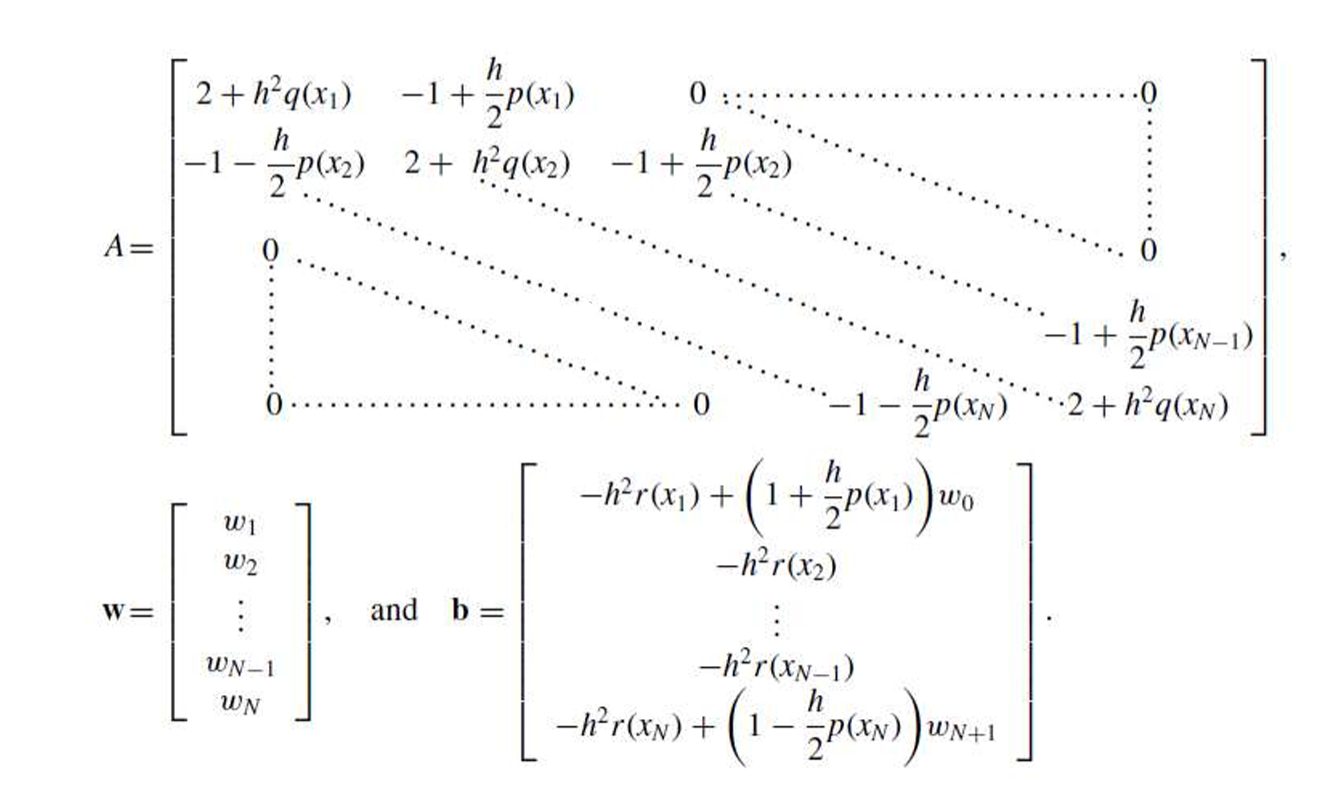
\includegraphics[width=1\linewidth]{pvc_sistema.png}
    \caption{Sistema tridiagonal}
    \label{fig:enter-label}
\end{figure}

Con los ejercicios queda mas claro, asi que chill. 


\subsection{Integración}
    \subsubsection{Trapecios}
    $$T(h) = \frac{h}{2} [f(a) + f(b) + 2\sum_{i = 1}^{N-1}f(x_{i})]$$
    
    \subsubsection{Simpson}
    $$
    S(h) = \frac{h}{3} [f(a) + f(b) + 2\sum_{k = 1}^{\frac{N-2}{2}}f(x_{2k}) + 4\sum_{k = 0}^{\frac{N-2}{2}}f(x_{2k + 1})]
    $$
    \subsubsection{Gauss}

    Tenemos la siguiente integral
    $$\int_{a}^{b} f(x) \approx \sum_{i = 0}^{n} w_if(x_i)$$

    Normalizamos de la siguiente manera: 
    $$x = \frac{(b-a)t ~+~ (b+a) }{2}$$
    $$dx = \frac{b-a}{2} dt$$

    Reemplazamos en la integral original y nos queda lo siguiente
    $$\int_{a}^{b} f(x) = \frac{b-a}{2}\int_{-1}^{1}f(\frac{(b-a)t ~+~ (b+a) }{2})dt$$